\documentclass{beamer}

\usepackage{amsmath}

\usetheme{AnnArbor}
\usecolortheme{crane}
\usefonttheme[onlymath]{serif}

\title{Deep Learning - Foundations and Concepts}
\subtitle{Chapter 5. Single-layer Networks: Classification}
\author{nonlineark@github}
\date{\today}

\begin{document}

\begin{frame}
    \titlepage
\end{frame}

\begin{frame}
    \frametitle{Outline}
    \tableofcontents
\end{frame}

\section{Discriminant Functions}

\begin{frame}
    \frametitle{Discriminant functions}
    \begin{itemize}
        \item The goal in classification is to take an input vector $x\in\mathbb{R}^{D}$ and assign it to one of $K$ discrete classes $\mathcal{C}_{k}$.
        \item A discriminant is a function that takes an input vector $x$ and assigns it to one of $K$ classes, denoted $\mathcal{C}_{k}$.
        \item We will restrict attention to linear discriminants, for which the decision surfaces are hyperplaines.
    \end{itemize}
\end{frame}

\begin{frame}
    \frametitle{Two classes}
    Taking a linear function of the input vector:
    \begin{equation*}
        y(x)=w^{T}x+w_{0}
    \end{equation*}
    \begin{itemize}
        \item An input vector is assigned to class $\mathcal{C}_{1}$ if $y(x)\ge{}0$ and to class $\mathcal{C}_{2}$ otherwise.
        \item The decision boundary is a $(D-1)$-dimensional hyperplane.
    \end{itemize}
\end{frame}

\begin{frame}
    \frametitle{Two classes}
    \begin{figure}
        \caption{The geometry of a linear discriminant function in two dimensions}
        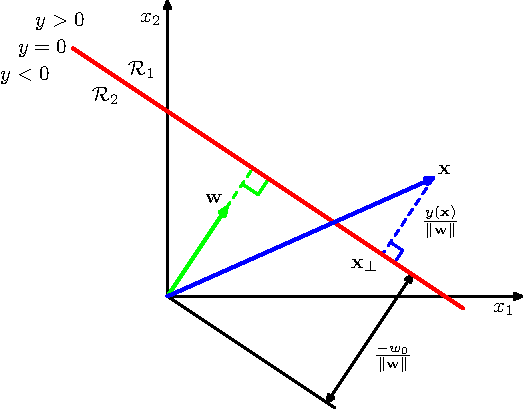
\includegraphics[height=0.6\textheight]{Figure_1.pdf}
    \end{figure}
\end{frame}

\begin{frame}
    \frametitle{Two classes}
    It's easy to see that:
    \begin{itemize}
        \item $w$ is orthogonal to the decision surface.
        \item $w$ points to the direction of the increase of $y$.
    \end{itemize}
    Also the value of $y(x)$ gives a signed measure of the perpendicular distance $r$ of the point $x$ from the decision surface:
    \begin{align*}
        x&=x_{\perp}+r\frac{w}{||w||} \\
        y(x)&=w^{T}x+w_{0}=w^{T}x_{\perp}+w_{0}+r||w||=r||w|| \\
        r&=\frac{y(x)}{||w||}
    \end{align*}
    In particular, the signed distance of the origin from the decision surface is given by $\frac{w_{0}}{||w||}$.
\end{frame}

\end{document}